\documentclass{beamer}
\usepackage{tikz}
\usepackage[utf8]{inputenc}
\usepackage[portuges]{babel}
\usepackage{utopia} %font utopia imported
\usepackage{listings}
\usetheme{Madrid}
\usecolortheme{default}


%------------------------------------------------------------
%This block of code defines the information to appear in the
%Title page
\title[(Shelf) Bin Packing 2D - 2SBP] %optional
{(Shelf) Bin Packing 2D - 2SBP}

\subtitle{Modelagem no CPLEX}

\author[Diego Ramon] % (optional)
{\scriptsize Diego Ramon \\
diego.ramon@eng.ci.ufpb.br}

\institute[UFPB]  % (optional)
{\\[1.0mm] 
 Universidade Federal da Paraíba\\
 Pós-Graduação em Informática\\ 
 Pesquisa Operacional
}

\date[PO 2019] % (optional)
{\tiny {14 de Junho de 2019}}



%End of title page configuration block
%------------------------------------------------------------



%------------------------------------------------------------
%The next block of commands puts the table of contents at the 
%beginning of each section and highlights the current section:

\AtBeginSection[]
{
  \begin{frame}
    \frametitle{Table of Contents}
    \tableofcontents[currentsection]
  \end{frame}
}
%------------------------------------------------------------


\begin{document}

\frame{\titlepage}
%---------------------------------------------------------
%This block of code is for the table of contents after
%the title page
\begin{frame}
\frametitle{\textbf{Agenda}}
	\hspace*{+4.0em}
	\footnotesize{ \tableofcontents }
\end{frame}

%---------------------------------------------------------

\section{Introdução}

\subsection{Informações do Artigo}

\begin{frame}
\frametitle {Informações do Artigo}

 \begin{itemize}
    \item Título: Algoritmo GRASP/VND para o problema clássico de empacotamento
tridimensional e bidimensional
    \item Autores: Anderson Zudio et al.
    \item Publicado em: Simpósio Brasileiro de Pesquisa Operacional (SBPO)
    \item Ano: 2017
    
 \end{itemize}

\end{frame}

\subsection{Definição do Problema}

\begin{frame}
\frametitle {Introdução}

    \begin{itemize}
    \item 
        O problema clássico bidimensional de empacotamento (2BP) consiste em empacotar ortogonalmente um conjunto de n itens retangulares caracterizados por sua largura $w_i$, altura $h_i$, $i \in S = {1, \dots, n}$, no menor número possível de caixas homogêneas de largura $W$ e altura $H$.
    \item Porém, esse problema é tratável via programação linear inteira, pois requer uma grande quantidade de variáveis binárias (não polinomial). Literatura predominante de soluções baseadas em meta-heurísticas.
    \end{itemize}
\end{frame}

\begin{frame}
\frametitle {Introdução}

    \begin{itemize}
    \item No entanto, esse problema se torna tratável via programação linear inteira com o uso de restrições de "prateleira". Pois permite obter um número polinomial de variáveis. 
    \end{itemize}
\end{frame}

\begin{frame}
    \frametitle{Introdução}
    \begin{figure}
    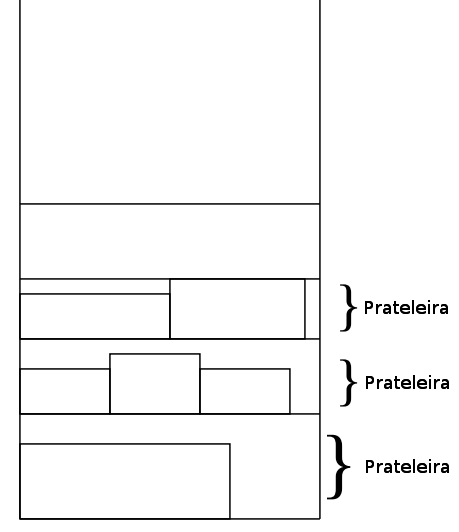
\includegraphics[scale=0.3]{sheft.png}
    \caption{Representação gráfica do problema.}
    \end{figure}
\end{frame}

\section{Modelagem}

\subsection{Hipóteses}

\begin{frame}
\frametitle {Hipóteses}

    \begin{enumerate}
    \item 
    O primeiro item (mais à esquerda) embalado em cada prateleira é o item mais alto em si;
    \item 
    A primeira prateleira (inferior), embalada em cada caixa / faixa, é a prateleira mais alta na caixa / faixa.
    \item 
    Os itens são ordenados, então $h_1 \geq h_2 \geq \dots \geq h_n $
    \end{enumerate}
\end{frame}

\subsection{Variáveis}
\begin{frame}
\frametitle {Variáveis}

{\small
\nonumber
\begin{align}
    \nonumber
    y_{i} & =
    \begin{cases}
        1 &\text{se prateleira $i$ inicializa bin $i$},\\
        0 &\text{caso contrário }
    \end{cases}  &  (&i = 1, \dots, n) \\
    \\
    q_{k} & =
    \begin{cases}
        1 &\text{se item $k$ inicializa prateleira $k$},\\
        0 &\text{caso contrário }
    \end{cases}  &  (&k = 1, \dots, n) \\
    \\
    x_{ij} &=
    \begin{cases}
        1 &\text{se item $j$ é empacotado na prateleira $i$},\\
        0 &\text{caso contrário }
    \end{cases}  &  (&i = 1, \dots, n-1;  j > i) \\
    q_{ki} &=
    \begin{cases}
        1 &\text{se prateleira $i$ é alocado para bin  $k$},\\
        0 &\text{caso contrário }
    \end{cases} &  (&k = 1, \dots, n-1; i > k) \\
\end{align}
}

\end{frame}

\subsection{Modelo}

\begin{frame}
\frametitle {Modelo}

A Equação (0) modelo a função objetivo que minimiza o número de bins usados.

{\small
\begin{align}
\min \quad
& \sum_{q=1}^{n} q_k 
\end{align} 
}

\end{frame}

\begin{frame}

A Equação (1) impõem que cada item seja empacotado exatamente uma vez, seja inicializando uma prateleira ou numa prateleira inicializada por um item anterior (mais alto).

\frametitle {Modelo}

{\small
\begin{align}
\quad
& \sum_{i=1}^{j-1} x_{ij} + y_j = 1 &  (j = 1, \dots, n)  
\end{align} 
}
\end{frame}

\begin{frame}

A Equação (2) impõem que cada prateleira seja usada seja alocada exatamente uma vez, seja inicializando uma bin ou em um bin inicializado por uma prateleira anterior (mais alta).

\frametitle {Modelo}

{\small
\begin{align}
\quad
& \sum_{k=1}^{i-1} z_{ki} + q_i = y_i  & (i = 1, \dots, n) 
\end{align} 
}
\end{frame}

\begin{frame}
A Equação (3) impõem a restrição de largura a cada prateleira usada.

\frametitle {Modelo}

{\small
\begin{align}
\quad
& \sum_{j=i+1}^{n} w_j x_{ij} \leq (W - w_i)y_i  & (i = 1, \dots, n-1) 
\end{align} 
}
\end{frame}

\begin{frame}

A Equação (4) impõem a restrição de altura a cada prateleira usada.

\frametitle {Modelo}

{\small
\begin{align}
\quad
& \sum_{i=k+1}^{n} h_i z_{ki} \leq (H - h_k)q_k  & (k = 1, \dots, n-1)
\end{align} 
}
\end{frame}

\begin{frame}
\setcounter{equation}{0}
\frametitle {Modelo}

{\small
\begin{align}
\min \quad
& \sum_{q=1}^{n} q_k \\
\text{sujeito a}\quad
& \sum_{i=1}^{j-1} x_{ij} + y_j = 1 &  (j = 1, \dots, n)  \\
& \sum_{k=1}^{i-1} z_{ki} + q_i = y_i  & (i = 1, \dots, n) \\
& \sum_{j=i+1}^{n} w_j x_{ij} \leq (W - w_i)y_i  & (i = 1, \dots, n-1) \\
& \sum_{i=k+1}^{n} h_i z_{ki} \leq (H - h_k)q_k  & (k = 1, \dots, n-1) \\
& x_{ij}, y_i, q_k, z_{ki} \in \{0,1\}
\end{align} 
}
\end{frame}

\section{Implementação}


\section{Resultados}

\begin{frame}


\begin{table}
    \tiny
    
    \begin{tabular}{| l | c | c | c | c | }
     \hline
    Classe & n & LB & Z & ILP \\
    \hline
    1 & 20 & 7,1 & 7,1 & 6,8 \\
      & 40 & 13,4 & 13,4 & 12,5 \\
      & 60 & 19,7 & 20,0 & 19,1 \\ 
      & 80 & 27,4 & 27,5 & 26,1 \\
      & 100 & 31,7 & 31,8 & 29,8 \\
    \hline
    2 & 20 & 1,0 & 1,0 & 1,0 \\
      & 40 & 1,9 & 1,9 & 1,0 \\
      & 60 & 2,5 & 2,5 & 1,4 \\ 
      & 80 & 3,1 & 3,1 & 1,8 \\
      & 100 & 3,9 & 3,9 & 1,9 \\
    \hline
     3 & 20 & 5,1 & 5,1 & 4,7 \\
      & 40 &  9,2 & 9,5 & 8,5 \\
      & 60 & 13,6 & 14,0 & 12,8 \\ 
      & 80 & 18,7 & 19,0 & 17,5 \\
      & 100 & 22,1 & 22,3 & 20,4 \\
    \hline
     4 & 20 & 1,0 & 1,0 & 1,0\\
      & 40 & 1,9 & 1,9 & 1,0\\
      & 60 & 2,3 & 2,5 & 1,2 \\ 
      & 80 & 3,0 & 3,2 & 1,6 \\
      & 100 & 3,7 & 3,8 & 1,8 \\
    \hline
     5 & 20 & 6,5 & 6,5 & 5,9 \\
      & 40 & 11,9 & 11,9 & 11,1 \\
      & 60 & 17,9 & 18,1 & 16,9 \\ 
      & 80 & 24,1 & 24,7 & 23,3 \\
      & 100 & 27,9 & 28,2 & 26,6 \\
    \hline \hline
    \end{tabular}
    \caption{Resultados  computacionais com Cplex}
\end{table}
\end{frame}

\section{Referências}

\begin{frame}
\frametitle {Referências}

    \begin{itemize}
    \item ZUDIO, Anderson, et al. Algoritmo GRASP/VND para o problema clássico de empacotamento tridimensional e bidimensional.
    \item Lodi, Andrea. (2019). Algorithms for Two-Dimensional Bin Packing and Assignment Problems. 
    \end{itemize}
\end{frame}

\end{document}